\documentclass[conference]{IEEEtran}

\usepackage[T1]{fontenc}
\usepackage{amsmath}
\usepackage{amssymb}
\usepackage{flushend}
\usepackage{booktabs}
\usepackage{cite}
\usepackage{graphicx}
\usepackage{multirow}
\usepackage[hidelinks]{hyperref}

\title{From Multi-Kernel Redundancy to Executable Sparsity: A Controlled Study of Conditional Computation in Lightweight Medical Segmentation}

\author{\IEEEauthorblockN{M Mohaiminul Islam}
\IEEEauthorblockA{Department of Computer Science and Telecommunication Engineering\\
Noakhali Science and Technology University}}

\begin{document}

\maketitle

\begin{abstract}
Lightweight multi-kernel segmentation networks keep several receptive fields by running every branch for every image. This paper studies whether some of that repeated work can be changed into real skipped computation without a large accuracy loss. MK-UNet is used as a controlled backbone. Only the aggregation of its $1\times1$, $3\times3$, and $5\times5$ depth-wise branches is changed: fixed summation, adaptive soft weighting, hard top-1 execution, and a secondary static ablation. The study covers three widths and six binary medical datasets, giving 72 completed single-seed runs. After adaptive pretraining and unequal-budget sparse fine-tuning, top-1 inference runs one of three branches per routed block. Forward hooks confirm that MK-UNet-T calls 10 of 30 possible branch convolutions; profiled FLOPs fall by 54.1\%, but batch-1 CPU latency falls by only 13.3\%. FLOP reductions fall to 42.4\% and 29.4\% for the wider models. This shows that useful sparsity depends on model width. Accuracy point estimates stay close on average, but they are descriptive because each setting uses one seed and sparse training receives extra optimization. The results show that conditional computation should be checked with real executed operations and measured runtime, not FLOPs alone.
\end{abstract}

\begin{IEEEkeywords}
Medical image segmentation, lightweight neural networks, conditional computation, dynamic routing, multi-kernel convolution.
\end{IEEEkeywords}

\section{Introduction}
U-shaped encoder--decoder networks remain a common foundation for medical image segmentation because they combine contextual features with high-resolution skip information~\cite{ronneberger2015unet}. More broadly, efficient vision networks increasingly use parallel kernels, multi-scale features, and attention branches to preserve several receptive fields. These designs improve representational flexibility, but usually execute the same collection of branches for every input. This raises a general deployment question: does every image require every available receptive field at every stage? For point-of-care and edge use, the answer must be evaluated through executed operations and realized latency rather than parameter count or nominal FLOPs alone.

MK-UNet addresses this regime with multi-kernel inverted residual blocks built from depth-wise convolutions and lightweight attention~\cite{rahman2025mkunet}. Its multi-kernel depth-wise convolution (MKDC) evaluates three parallel branches and sums them,
\begin{equation}
    F(x)=F_1(x)+F_3(x)+F_5(x),
    \label{eq:fixed}
\end{equation}
where the subscript denotes kernel size. The design supplies several receptive fields, but it also assumes that all three are equally useful for every input and stage. This creates a specific gap: the architecture is lightweight, yet its defining multi-kernel computation is unconditional.

This work treats MK-UNet as a controlled test bed, not as a place to claim a completely new routing algorithm. The U-shaped topology, attention gates, channel widths, and output heads stay unchanged; only MKDC aggregation changes. Soft weighting tests input-conditioned receptive fields, hard top-1 dispatch tests real skipped computation, and a static $\{3,5\}$ ablation tests whether a small routing diagnostic relates to fixed branch removal.

The study asks three questions: (RQ1) does adaptive routing retain the fixed model's aggregate accuracy under matched local training; (RQ2) can top-1 dispatch physically skip branch computation and reduce measured latency; and (RQ3) how does the accuracy--computation trade-off change with model width and dataset?

The goal is not to propose a universally better segmentation architecture or a new routing algorithm. Instead, this paper studies when existing multi-kernel computation can become executable sparsity. MK-UNet gives a small and controlled example of this broader question.

The contributions are threefold:
\begin{itemize}
    \item This paper studies whether repeated multi-kernel computation in an ultra-light medical segmenter can become real skipped computation while the rest of the backbone stays unchanged.
    \item Fixed, adaptive, and post-pretraining sparse settings are evaluated in 72 runs across three widths and six datasets. Static branch removal is kept only as a secondary exploratory ablation.
    \item Physical branch skipping is checked with hooks. Profiled FLOPs are separated from CPU latency, and the reason why the skippable fraction falls as channel width grows is derived.
\end{itemize}

\section{Related Work}
This section places the work in three simple contexts. First, it reviews efficient medical segmentation models. Second, it discusses multi-kernel designs that use more than one receptive field. Third, it connects the study to conditional computation and runtime-aware model design.

\subsection{Efficient Medical Image Segmentation}
U-Net established the encoder--decoder and skip-connection pattern used by many biomedical segmentation systems~\cite{ronneberger2015unet}. MobileNetV2 subsequently showed how inverted residuals and depth-wise filtering reduce computation in mobile networks~\cite{sandler2018mobilenetv2}. Medical segmentation designs have combined these efficiency principles with different context mechanisms. UNeXt mixes convolutional stages with tokenized MLP blocks~\cite{valanarasu2022unext}; EGE-UNet uses grouped multi-axis attention and aggregation bridges~\cite{ruan2023egeunet}; and CMUNeXt uses large depth-wise kernels, inverted bottlenecks, and skip fusion~\cite{tang2024cmunext}. These architectures demonstrate that useful context can be recovered under tight parameter budgets, although their principal inference graphs remain fixed for a chosen model.

MK-UNet is the closest basis for this study. It combines MobileNet-style inverted residuals with parallel $1\times1$, $3\times3$, and $5\times5$ depth-wise kernels and decoder attention, reporting five widths from 0.027M to 3.76M parameters~\cite{rahman2025mkunet}. Instead of adding a new encoder or decoder, this work keeps that architecture and asks one question: must its parallel kernels run for every input?

\subsection{Multi-Kernel Receptive Fields}
Mixed-kernel designs obtain several receptive fields in different ways. MixConv splits channels across depth-wise kernels of different sizes, giving a static and hardware-friendly mixture~\cite{tan2019mixconv}. Selective Kernel Networks run several branches and use softmax attention to adapt the effective receptive field to the input~\cite{li2019sknet}. MK-UNet instead sums all depth-wise branches with equal weights~\cite{rahman2025mkunet}. The adaptive arm in this paper is related to selective-kernel attention, but it also has a diagnostic role: it supplies the router used for hard top-1 execution and the static $\{3,5\}$ comparison. The main difference is simple: soft attention alone does not save branch computation; saving computation requires an inference path that never calls unselected convolutions.

\subsection{Conditional Computation, Pruning, and Runtime}
CondConv constructs example-dependent kernels from learned experts~\cite{yang2019condconv}, while dynamic convolution applies input-conditioned attention to parallel kernels~\cite{chen2020dynamicconv}. SkipNet learns whether residual blocks should execute~\cite{wang2018skipnet}, and dynamic routing for semantic segmentation selects scale-dependent network paths~\cite{li2020dynamicrouting}. Structured pruning instead learns one fixed compact graph; network slimming is a representative channel-level approach~\cite{liu2017slimming}. MK-UNet-CC evaluates both categories through a dynamic top-1 model and a static two-branch model.

Dynamic operators have also been used in medical segmentation. LightAWNet combines dynamic convolution with adaptive weighting~\cite{wang2025lightawnet}; an auto-dynamic convolution and location-attention model targets adaptive feature extraction~\cite{wang2025adlaformer}; and SEDyConv improves dynamic convolution across spatial and kernel dimensions for multi-organ CT segmentation~\cite{hao2025sedyconv}. These studies support input-conditioned feature extraction in medical images. This paper is different in two ways: the dynamic unit is inserted into an existing ultra-lightweight baseline without changing its topology, and the efficiency claim requires physical branch non-execution plus measured latency, not only adaptive fusion.

Table~\ref{tab:novelty} makes this boundary clear. SKNet and Dynamic Convolution adapt kernel mixtures but still run dense expert evaluation or aggregation~\cite{li2019sknet,chen2020dynamicconv}. SkipNet gives executable conditional computation at the residual-block level, but it was tested on natural-image recognition~\cite{wang2018skipnet}. LightAWNet evaluates dynamic filtering for medical segmentation, but it does not report input-conditioned branch non-execution~\cite{wang2025lightawnet}. The contribution of this paper is therefore not soft routing itself; it is the controlled change of an existing medical segmenter's parallel multi-kernel block into verified branch-level sparsity.

\begin{table}[t]
\caption{Position relative to closely aligned conditional methods. ``Skip'' denotes reported non-execution of an input-conditioned convolutional branch or block; N/R means not reported.}
\label{tab:novelty}
\centering
\scriptsize
\setlength{\tabcolsep}{3.2pt}
\begin{tabular}{lcccl}
\toprule
Method & Dynamic & Medical & Skip & Conditional unit \\
\midrule
SKNet~\cite{li2019sknet} & Yes & No & No & kernel fusion \\
Dynamic Conv.~\cite{chen2020dynamicconv} & Yes & No & No & kernel aggregation \\
SkipNet~\cite{wang2018skipnet} & Yes & No & Yes & residual block \\
LightAWNet~\cite{wang2025lightawnet} & Yes & Yes & N/R & dynamic kernel \\
This study & Yes & Yes & Yes & MKDC branch \\
\bottomrule
\end{tabular}
\end{table}

Less arithmetic does not always mean the same amount of speedup. Spatially dynamic convolutions need careful gather--scatter implementations~\cite{verelst2020spatial}, and ShuffleNet V2 shows that memory access, parallelism, and hardware details matter along with FLOP counts~\cite{ma2018shufflenetv2}. This motivates the use of profiler output, CPU timing, and hook-based branch counts in this work. Unlike broad path-routing methods, the action space here has only three explicit depth-wise branches inside an ultra-lightweight block, so the source of both savings and overhead can be inspected directly.

\section{Method}
This section describes only the part of MK-UNet that is changed. The encoder, decoder, attention gates, and output head stay the same. The study changes how the three MKDC branches are combined and then checks whether one branch can be executed while the other two are skipped. Figure~\ref{fig:architecture} separates the unchanged MK-UNet topology from the conditional MKDC block and its three execution modes.

\subsection{Adaptive Soft Routing}
For feature map $x\in\mathbb{R}^{C\times H\times W}$, the router applies global average pooling followed by two $1\times1$ convolutions and ReLU. With logits $z(x)$, temperature $T$, and $K=3$ branches, it produces
\begin{equation}
\begin{aligned}
    a_k(x)&=K\frac{\exp(z_k(x)/T)}{\sum_j\exp(z_j(x)/T)},\\
    F_{\mathrm{soft}}(x)&=\sum_k a_k(x)F_k(x).
\end{aligned}
    \label{eq:soft}
\end{equation}
The final router layer is zero-initialized, so $a_k=1$ initially and (\ref{eq:soft}) exactly matches the scale of the fixed sum in (\ref{eq:fixed}). The router bottleneck reduction is four. Soft routing remains dense because all branches are evaluated.

\subsection{Sparse Top-1 Routing}
The hard path selects $k^*=\arg\max_k a_k(x)$ and sets the other weights to zero. The selected weight is rescaled so the hard weights sum to $K$, preventing a threefold activation shrink when moving from soft to hard routing. Training uses a straight-through estimator: the forward pass uses hard weights, gradients use the soft weights, and all branches are evaluated so their parameters receive gradients. A linear 40-epoch ramp blends soft and hard routing. At inference, the implementation dispatches only the selected branch; batch size one has a dedicated path without gather--scatter overhead.

Each sparse run is warm-started from the best validation checkpoint of its corresponding 200-epoch adaptive run and then fine-tuned for 120 epochs. Accordingly, sparse Dice describes performance after adaptive pretraining; it is not an equal-training-budget accuracy comparison with the from-scratch arms. The inference graphs and measured inference costs remain directly comparable.

\subsection{Exploratory Branch-Removal Analysis}
A pilot analysis of a trained ClinicDB soft router measured the norm share and pairwise cosine similarity of branch outputs. Across ten routed blocks and three images, the mean shares of the $1$, $3$, and $5$ branches were 0.260, 0.320, and 0.420, and mean off-diagonal cosine similarity was 0.389. Removing the $1\times1$ branch caused the smallest relative output change in that diagnostic. Therefore, a static $\{3,5\}$ model is trained from scratch as a secondary exploratory ablation. It is not presented as a pruning method or an optimal kernel-selection rule.
Figure~\ref{fig:diagnostic} separates this offline analysis from the forward architecture.

\begin{figure*}[t]
\centering
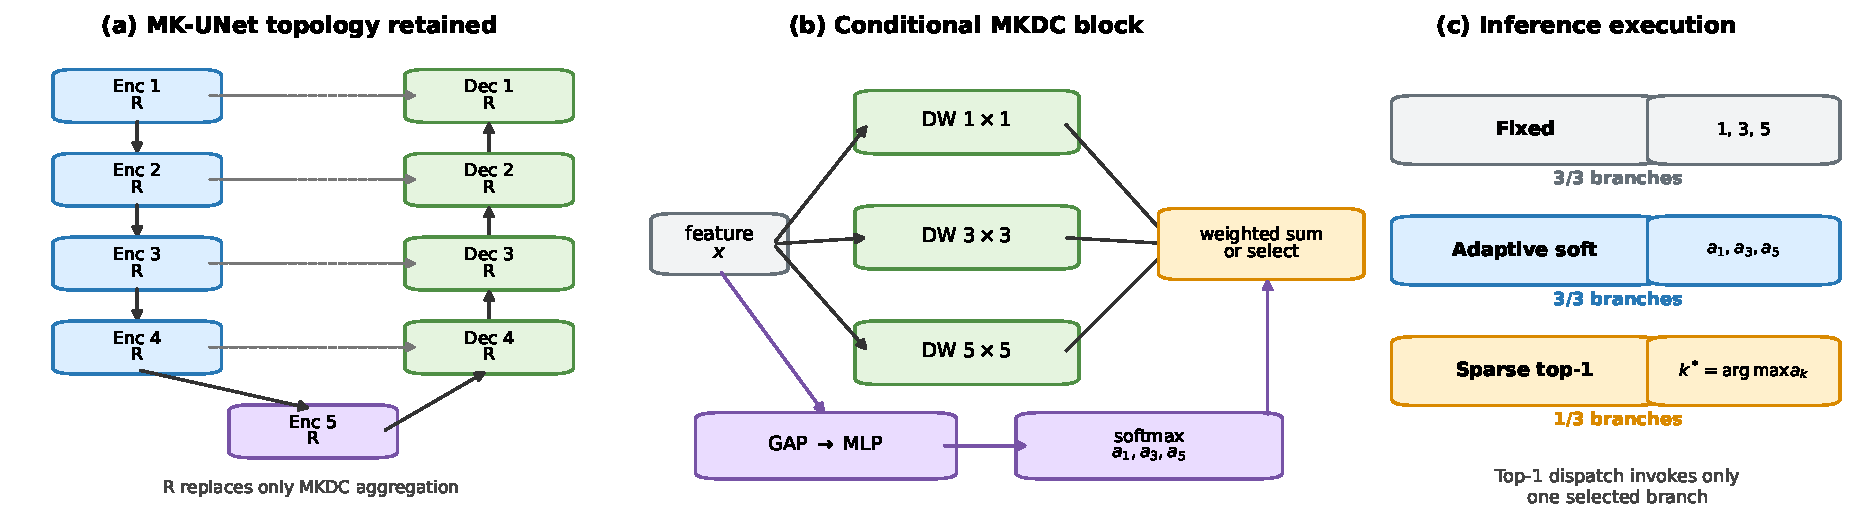
\includegraphics[width=0.98\textwidth]{figures/conditional_routing_architecture.pdf}
\caption{Controlled modification of MK-UNet. The topology is retained and only MKDC aggregation is changed. Fixed and adaptive-soft inference execute all three depth-wise branches; sparse top-1 dispatch invokes only the selected branch.}
\label{fig:architecture}
\end{figure*}

\begin{figure*}[t]
\centering
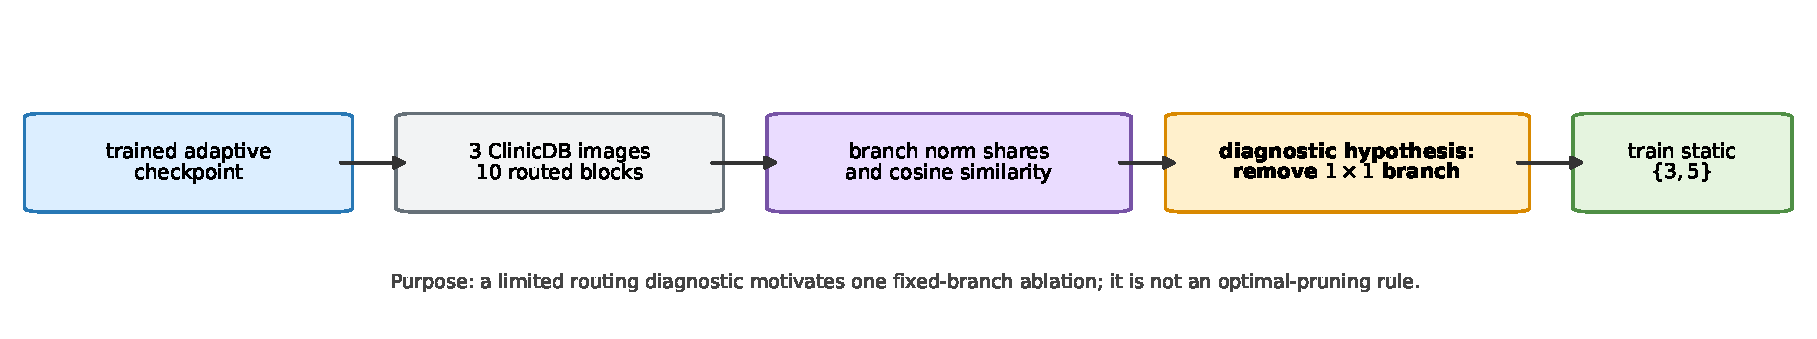
\includegraphics[width=0.92\textwidth]{figures/diagnostic_static_ablation.pdf}
\caption{Secondary exploratory branch-removal analysis. Statistics from three ClinicDB images motivate a $\{3,5\}$ hypothesis that is trained from scratch. This limited diagnostic is not a pruning rule.}
\label{fig:diagnostic}
\end{figure*}

\section{Experimental Protocol}
This section explains how the comparison is made. It lists the datasets, model sizes, training settings, evaluation rule, and efficiency measurement. The goal is to make every reported number traceable to a clear run setting.

\subsection{Datasets and Splits}
This study uses the six binary datasets from MK-UNet: BUSI breast ultrasound, ClinicDB and ColonDB polyp images, ISIC18 skin lesions, DSB18 nuclei, and EM microscopy structures~\cite{rahman2025mkunet}. Table~\ref{tab:data} reports the prepared split counts. Polyp images are resized to $352\times352$; all others use $256\times256$.

Figure~\ref{fig:datasets} illustrates the substantial appearance and target-geometry variation covered by the study. To avoid selecting unusually large or visually convenient targets, each displayed test example is chosen deterministically as the sample whose foreground fraction is closest to that dataset's test-split median.

\begin{figure*}[t]
\centering
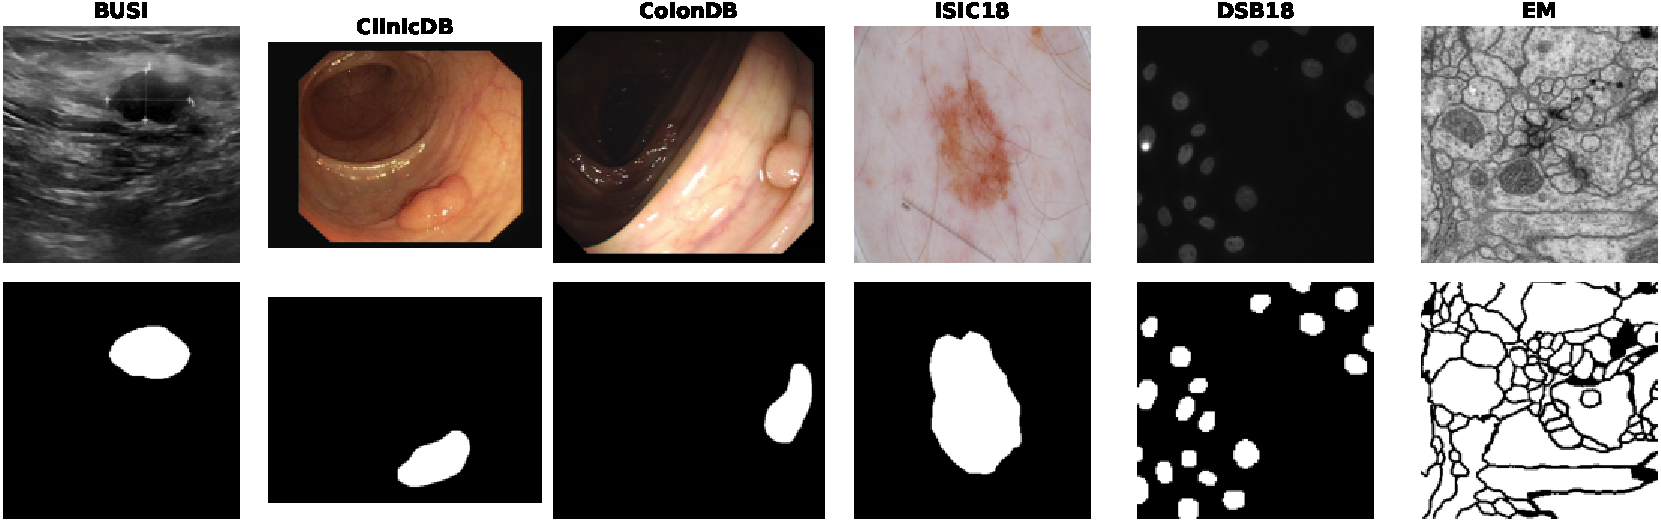
\includegraphics[width=0.98\textwidth]{figures/dataset_examples.pdf}
\caption{Representative prepared test examples. The top row shows input images and the bottom row shows their ground-truth masks. From left to right: BUSI, ClinicDB, ColonDB, ISIC18, DSB18, and EM.}
\label{fig:datasets}
\end{figure*}

\begin{table}[t]
\caption{Prepared 80:10:10 dataset splits.}
\label{tab:data}
\centering
\footnotesize
\begin{tabular}{lrrr}
\toprule
Dataset & Train & Val. & Test \\
\midrule
BUSI     & 518  & 65  & 64  \\
ClinicDB & 489  & 61  & 62  \\
ColonDB  & 303  & 38  & 38  \\
ISIC18   & 2075 & 259 & 260 \\
DSB18    & 536  & 67  & 67  \\
EM       & 24   & 3   & 3   \\
\bottomrule
\end{tabular}
\end{table}

\subsection{Models and Training}
This work evaluates MK-UNet-T (Tiny), MK-UNet-S (Small), and standard MK-UNet (largest evaluated), with channel sequences $[4,8,16,24,32]$, $[8,16,32,48,80]$, and $[16,32,64,96,160]$, respectively. The official standard name is kept because the unevaluated architecture also defines L and XL variants. For every scale--dataset pair, fixed $\{1,3,5\}$, static $\{3,5\}$, adaptive-soft, and sparse-top-1 settings are trained with seed 42. This gives $3\times6\times4=72$ completed runs.

Fixed, exploratory-static, and adaptive models train for 200 epochs with batch size 8, AdamW, learning rate $5\times10^{-4}$, weight decay $10^{-4}$, cosine decay, and gradient clipping at 0.5. Sparse fine-tuning uses learning rate $3\times10^{-4}$. Training evaluates image scales $\{0.75,1,1.25\}$ and uses rotations up to $90^\circ$, horizontal and vertical flips, and resizing. The loss is weighted binary cross-entropy plus weighted IoU. The checkpoint is selected by validation Dice; the reported value is test Dice at that checkpoint. Predictions are resized to the original image size, normalized per image, and thresholded at 0.5.

The sweep was divided across three Windows CPU machines. Artifact snapshots report PyTorch 1.11.0, 24 CPU threads, and the same Intel processor family; Machine A used Python 3.8 and Machines B/C used Python 3.9. Arms belonging to one scale--dataset unit stayed on the same machine, so within-unit comparisons do not cross hardware.

\subsection{Evaluation and Statistical Scope}
For binary prediction $p$ and target $y$, the reported Dice is summarized by
\begin{equation}
    \mathrm{Dice}(p,y)=\frac{2\sum_i p_i y_i+\epsilon}
    {\sum_i p_i+\sum_i y_i+\epsilon}.
    \label{eq:dice}
\end{equation}
Dataset values are computed by the repository evaluation pipeline after per-image normalization and thresholding. Scale means average the six dataset scores equally, and the overall result averages all 18 scale--dataset units; large datasets therefore do not dominate by pixel or image count. Comparisons between variants are paired within each unit. Every cell contains one seed. Because the base paper itself reports roughly 1--4 Dice points of run-to-run standard deviation, sub-point differences in this study must be interpreted descriptively~\cite{rahman2025mkunet}. Therefore, significance tests and confidence intervals are omitted. Published MK-UNet numbers are shown separately from matched local comparisons.

\subsection{Efficiency Measurement}
FLOPs are profiled at $256\times256$ using THOP. Because profiler counts do not capture all routing and dispatch costs, batch-1 CPU latency is also measured. The latency audit uses PyTorch 1.11.0, 16 CPU threads, three warm-up passes, and ten timed passes. Forward hooks independently count every depth-wise branch call.

\section{Results}
This section reports the results in four steps. It first explains why the local fixed model is used as the main control. It then compares segmentation accuracy across scales and datasets, checks execution and efficiency, and finally summarizes the saved training artifacts.

\subsection{Reproduction Context}
Before the extension, the released MK-UNet-T pipeline produced 91.09 Dice on ClinicDB and 78.32 on ColonDB, compared with 91.26 and 85.03 in the base paper~\cite{rahman2025mkunet}. The first result is close; the second is not an exact reproduction. Also, the extension protocol uses repository-local settings such as augmentation, batch size 8, and learning rate $5\times10^{-4}$, while the base paper reports no augmentation, batch size 16, and learning rate $10^{-4}$. Therefore, the locally trained fixed arm is treated as the control, and this paper does not claim direct superiority over published MK-UNet values.

Table~\ref{tab:papercomparison} gives descriptive deployment context. After adaptive pretraining, sparse fine-tuning gives scale means 0.65--0.83 Dice points below the published values while removing 29.4--54.1\% of profiled inference FLOPs. The standard exploratory-static model is only 0.19 points below the paper mean, but its parameter reduction is only 1.1\%. Because the base paper reports five-run averages and this set of runs contains one seed under different training settings, these values are context rather than matched experimental deltas.

\begin{table}[t]
\caption{Published versus local mean Dice. Sparse scores follow adaptive pretraining and unequal-budget fine-tuning. T/S/Standard denote Tiny/Small/standard MK-UNet; $\Delta$ is sparse minus paper and Save is local sparse FLOP reduction.}
\label{tab:papercomparison}
\centering
\scriptsize
\setlength{\tabcolsep}{3.2pt}
\begin{tabular}{lrrrrrrr}
\toprule
Scale & Paper & Fixed & Static & Adapt. & Sparse & $\Delta$ & Save \\
\midrule
T    & 87.87 & 86.92 & 86.35 & 87.31 & 87.04 & -0.83 & 54.1\% \\
S    & 89.10 & 88.60 & 88.98 & 88.71 & 88.42 & -0.68 & 42.4\% \\
Standard & 89.75 & 89.51 & 89.56 & 89.25 & 89.10 & -0.65 & 29.4\% \\
\bottomrule
\end{tabular}
\end{table}

\subsection{Cross-Scale Segmentation Accuracy}
Table~\ref{tab:allresults} reports all completed runs. The from-scratch fixed, exploratory-static, and adaptive arms share a 200-epoch budget. Over their 18 matched units, adaptive soft routing is 0.08 Dice points above fixed and exploratory-static is 0.04 points below. Sparse top-1, evaluated only after adaptive pretraining and 120 additional epochs, is 0.15 points below fixed on average. Static, adaptive, and sparse point estimates exceed fixed in 13, 12, and 8 units, respectively. These are single-seed descriptive counts, not statistically significant wins or non-inferiority evidence.

\begin{table*}[t]
\caption{Single-seed test Dice (\%) at the best validation checkpoint. T/S/Standard are Tiny/Small/standard MK-UNet; F/P/A/S are fixed, exploratory-static, adaptive, and post-pretraining sparse. Sparse is not an equal-budget arm; bold is the row maximum.}
\label{tab:allresults}
\centering
\footnotesize
\setlength{\tabcolsep}{3.6pt}
\begin{tabular}{llrrrr|llrrrr|llrrrr}
\toprule
Scale & Dataset & F & P & A & S & Scale & Dataset & F & P & A & S & Scale & Dataset & F & P & A & S \\
\midrule
T & BUSI     & 78.11 & \textbf{78.24} & 76.89 & 76.68 &
S & BUSI     & 79.03 & \textbf{80.42} & 79.40 & 80.21 &
Standard & BUSI  & 81.05 & 78.58 & 79.25 & \textbf{82.28} \\
T & ClinicDB & 90.32 & \textbf{91.62} & 91.53 & 90.85 &
S & ClinicDB & 92.24 & 93.23 & \textbf{93.25} & 92.85 &
Standard & ClinicDB & 93.81 & \textbf{93.86} & 93.55 & 92.35 \\
T & ColonDB  & 81.86 & 77.29 & 84.16 & \textbf{85.17} &
S & ColonDB  & \textbf{88.63} & 87.24 & 86.75 & 85.42 &
Standard & ColonDB & 89.43 & \textbf{91.30} & 90.19 & 89.28 \\
T & ISIC18   & 89.81 & 89.24 & \textbf{90.25} & 89.59 &
S & ISIC18   & 89.46 & \textbf{90.35} & 89.78 & 89.83 &
Standard & ISIC18 & 89.38 & \textbf{89.88} & 89.76 & 89.63 \\
T & DSB18    & 90.05 & \textbf{90.08} & 89.59 & 89.27 &
S & DSB18    & 90.33 & 90.30 & \textbf{90.52} & 90.13 &
Standard & DSB18 & 90.63 & \textbf{90.88} & 90.67 & 89.95 \\
T & EM       & 91.35 & \textbf{91.64} & 91.43 & 90.68 &
S & EM       & 91.94 & 92.31 & \textbf{92.54} & 92.08 &
Standard & EM    & 92.76 & \textbf{92.89} & 92.07 & 91.12 \\
\midrule
\multicolumn{2}{l}{Mean over six} & 86.92 & 86.35 & \textbf{87.31} & 87.04 &
\multicolumn{2}{l}{Mean over six} & 88.60 & \textbf{88.98} & 88.71 & 88.42 &
\multicolumn{2}{l}{Mean over six} & 89.51 & \textbf{89.56} & 89.25 & 89.10 \\
\bottomrule
\end{tabular}
\end{table*}

Figure~\ref{fig:deltas} makes the heterogeneity explicit. The largest positive change is post-pretraining sparse MK-UNet-T on ColonDB ($+3.31$), while the corresponding exploratory-static model loses 4.57 points. On standard MK-UNet/ColonDB, the exploratory-static model instead gains 1.86 points. Such reversals argue against a scale- or dataset-independent ranking.

\begin{figure*}[t]
\centering
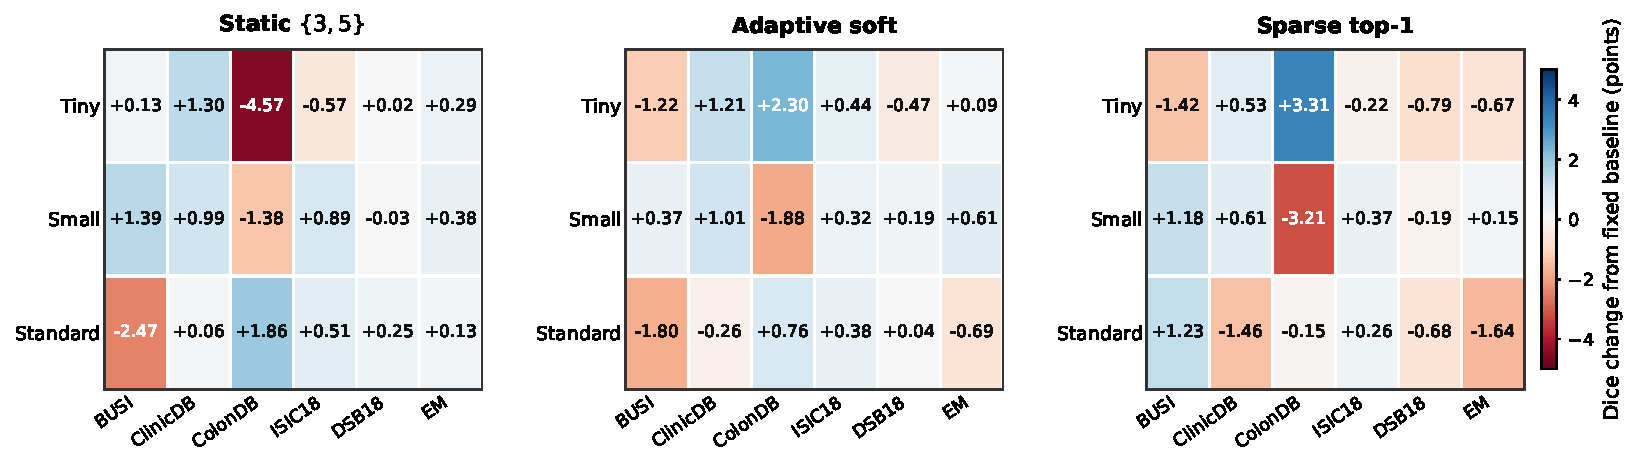
\includegraphics[width=0.98\textwidth]{figures/cross_scale_dice_delta.pdf}
\caption{Dice change from fixed $\{1,3,5\}$. Sparse values follow additional adaptive pretraining and are descriptive rather than equal-budget comparisons. Blue is higher and red is lower.}
\label{fig:deltas}
\end{figure*}

\begin{table}[t]
\caption{Aggregate single-seed accuracy over 18 units. Sparse follows adaptive pretraining. ``Higher'' counts a positive point difference; ``within 1'' counts differences no worse than $-1.0$.}
\label{tab:aggregate}
\centering
\footnotesize
\begin{tabular}{lrrrr}
\toprule
Variant & Mean & $\Delta$F & Higher & Within 1 \\
\midrule
Fixed $\{1,3,5\}$ & 88.34 & --    & --    & --    \\
Static $\{3,5\}$  & 88.30 & -0.04 & 13/18 & 15/18 \\
Adaptive soft      & 88.42 & +0.08 & 12/18 & 15/18 \\
Sparse (post-pre.) & 88.19 & -0.15 &  8/18 & 14/18 \\
\bottomrule
\end{tabular}
\end{table}

The direction and magnitude of the changes answer RQ1 and RQ3 more clearly than the overall mean. Exploratory-static differences range from $-4.57$ to $+1.86$ points, and adaptive differences range from $-1.88$ to $+2.30$. Post-pretraining sparse differences span $-3.21$ to $+3.31$. Median changes are $+0.19$, $+0.26$, and $-0.17$, respectively. The dispersion indicates that branch utility depends jointly on image domain, width, and learned features.

\subsection{Execution and Efficiency}
At batch size one, hooks find ten routers and 30 possible depth-wise branch calls in MK-UNet-T. Sparse top-1 executes exactly ten and skips 20; training mode executes all branches as required by the straight-through estimator. Table~\ref{tab:efficiency} shows that this lowers profiled FLOPs by 54.1\%. On the measured CPU, latency falls from 53.59 to 46.44~ms (13.3\%). Soft routing increases latency to 57.52~ms. The gap between FLOP and latency reductions demonstrates that global pooling, router layers, Python-level dispatch, and non-branch operations are material at this scale.

The width dependence can be derived from the implemented inverted-residual block. For expansion ratio two and channel width $C$, the three depth-wise kernels contribute approximately
\begin{equation}
    HW(2C)(1^2+3^2+5^2)=70CHW,
    \label{eq:dwcost}
\end{equation}
whereas the expansion and projection point-wise convolutions contribute approximately $4C^2HW$. Top-1 routing can remove two thirds of the first term but none of the quadratic term. The maximum skippable fraction therefore decreases as $C$ grows, even before router and dispatch overhead are counted. This explains the measured trend: savings fall from 54.1\% for T to 42.4\% for S and 29.4\% for standard MK-UNet, while router parameter overhead rises from 11.7\% to 17.7\%.

\begin{table}[t]
\caption{Complexity at $256\times256$. T/S/Standard are Tiny/Small/standard MK-UNet (largest evaluated). Router parameters apply to adaptive and sparse; latency is measured only for T.}
\label{tab:efficiency}
\centering
\scriptsize
\setlength{\tabcolsep}{3.4pt}
\begin{tabular}{lrrrrrr}
\toprule
Scale & Fixed P & $\{3,5\}$ P & Router P & F GF & S GF & Save \\
\midrule
T    & 27,384  & 26,550  & 30,588  & .0668 & .0307 & 54.1\% \\
S    & 93,050  & 91,304  & 107,382 & .1323 & .0762 & 42.4\% \\
Standard & 315,566 & 312,092 & 371,562 & .3275 & .2314 & 29.4\% \\
\bottomrule
\end{tabular}
\vspace{2pt}

\begin{tabular}{lrrr}
\toprule
T inference & Params & GFLOPs & CPU ms \\
\midrule
Fixed         & 27,384 & .0668 & 53.59 \\
Adaptive soft & 30,588 & .0677 & 57.52 \\
Sparse top-1  & 30,588 & .0307 & 46.44 \\
\bottomrule
\end{tabular}
\end{table}

\subsection{Convergence and Artifact Audit}
The saved histories provide a second check on the sweep. Mean best-validation epochs over the 18 runs are 141.0 for fixed, 151.8 for static, 128.6 for adaptive, and 75.8 of the 120 fine-tuning epochs for sparse. Broken down by scale, sparse peaks at epochs 81.2, 91.2, and 55.0 for T, S, and standard, respectively; the corresponding adaptive means are 143.8, 142.5, and 99.5. These values do not establish faster learning because sparse starts from an adaptive checkpoint, but they show that its reported score is not simply the final epoch of fine-tuning.

The 72 result records account for approximately 1100.7 aggregate CPU training hours: 306.3 fixed, 262.1 static, 334.2 adaptive, and 198.1 sparse fine-tuning hours. A sparse result therefore inherits its paired adaptive cost; the combined adaptive-plus-sparse path accounts for 532.3 hours. Wall-clock totals are reported for auditability, not used as a cross-machine efficiency metric. Each completed run directory stores the configuration, epoch history, result, checkpoint, and environment snapshot. The executable audit also records five passed sparse-routing checks and zero failures, including train/evaluation consistency and branch-hook counts. Together, these artifacts support exact tracing from every table entry to its run, while the single-seed limitation remains explicit.

\section{Discussion}
The principal finding is a boundary on when conditional multi-kernel computation pays, not a universally superior segmentation variant. Under the matched from-scratch budget, adaptive soft routing differs from fixed by only $+0.08$ points overall. After adaptive pretraining, sparse top-1 gives a similar aggregate point estimate while discarding two branches at every routed block. That observation concerns post-pretraining performance, not training efficiency or equal-budget accuracy. The exploratory-static result is secondary: it tests a branch-removal hypothesis but is not part of the central conditional-execution claim.

Relative to the published reference, the defensible claim is an accuracy--computation trade-off rather than improved Dice. The post-pretraining sparse scale means are less than one point below the base-paper means while saving 29.4--54.1\% of local fixed-graph FLOPs. This is not a controlled head-to-head result: the base values average five runs, while the local values are single runs with different preparation and optimization settings. The reported 1--4 point run-to-run variation in the base paper further cautions against ranking sub-point gaps.

The efficiency evidence is stronger and easier to explain. Hooks prove that branches are not merely masked after execution, and measured CPU latency confirms a real speedup for MK-UNet-T. Still, a 54.1\% FLOP reduction becomes only a 13.3\% latency reduction. Wider variants reduce the skippable fraction because point-wise convolutions dominate. Conditional routing should therefore be evaluated jointly with channel width, runtime, batch size, and deployment backend.

The deployment implications depend on hardware. Batch-1 edge CPUs can potentially benefit from avoiding two sequential branch calls, as the measured T result suggests. GPUs may realize a smaller gain because small kernels, launch overhead, and sample-wise divergence can outweigh arithmetic savings, especially for batched inference. Mobile NPUs commonly favor static compiled graphs; top-1 dispatch may therefore require compiler-supported conditional operators or separately compiled branch subgraphs. The exploratory-static $\{3,5\}$ graph avoids dispatch overhead but cannot adapt per input. These are implementation implications, not measured GPU or NPU results.

The exploratory branch-removal result remains deliberately limited. Router statistics suggested that the $1\times1$ branch had the smallest norm share in one ClinicDB pilot, and the resulting $\{3,5\}$ graph attains the strongest point estimate in 13 units. Its large T/ColonDB failure shows that three images cannot identify a universally removable branch. The result is evidence about the limits of the diagnostic, not a pruning recommendation; any deployment rule would need validation-domain selection.

Several limitations bound the claims. First, all 72 runs use one seed. Medical segmentation scores can vary by several Dice points across seeds, so differences below one point should not be interpreted as stable rankings. Second, sparse models inherit 200 adaptive epochs and receive 120 further epochs; training cost is larger and accuracy budgets are unequal. Third, the exploratory-static hypothesis uses only three ClinicDB images. Fourth, the test split was evaluated after every epoch, although checkpoint selection used validation Dice; future work should seal test data until model selection is complete. Fifth, latency is a short CPU-only benchmark without variance estimates, and THOP omits some elementwise and dispatch operations. No target mobile, GPU, or clinical-device benchmark is included.

The next study should repeat the matched arms over multiple seeds, train sparse models under a controlled total budget, select pruning rules using validation data only, and measure latency distributions on the intended deployment hardware. A fused sparse kernel would also test how much of the current FLOP--latency gap is an implementation artifact.

\section{Conclusion}
This controlled study asks whether MK-UNet's multi-kernel redundancy can become executable sparsity. Across 72 runs, the matched adaptive arm stays close to the fixed control on average, with clear scale--dataset variation. After adaptive pretraining, top-1 dispatch runs one third of the routed branches and reduces profiled FLOPs by 29.4--54.1\%. Hooks verify non-execution, and MK-UNet-T shows a 13.3\% batch-1 CPU latency reduction. The cost model explains why the benefit becomes smaller as width grows. These results show that conditional computation should be evaluated at the execution level rather than through FLOPs alone. The contribution is an empirical and explainable study of conditional computation in a lightweight medical backbone, not a claim of state-of-the-art segmentation accuracy.

\section*{Acknowledgment}
Acknowledgment text will be added before submission.

\bibliographystyle{IEEEtran}
\bibliography{references}

\end{document}
